\documentclass[aspectratio=169,11pt]{beamer}
\usepackage[T1]{fontenc}
\usepackage{lmodern}
\usepackage{amsmath,amssymb}
\usepackage{booktabs,tabularx,array}
\usepackage{graphicx}
\usepackage{tikz}
\usetikzlibrary{arrows.meta,positioning,calc,fit}
\graphicspath{{figures/}}

% ---------------------------------------------------------------- look
\definecolor{ink}{HTML}{1F2328}
\definecolor{muted}{HTML}{6B7280}
\definecolor{flight}{HTML}{2A78D6}
\definecolor{twin}{HTML}{EB6834}
\definecolor{truth}{HTML}{6250D6}
\definecolor{other}{HTML}{1BAF7A}
\definecolor{panel}{HTML}{F3F5F8}
\setbeamercolor{normal text}{fg=ink}
\setbeamercolor{frametitle}{fg=ink,bg=white}
\setbeamercolor{title}{fg=ink}
\setbeamercolor{structure}{fg=flight}
\setbeamercolor{alerted text}{fg=twin}
\setbeamercolor{block title}{fg=white,bg=flight}
\setbeamercolor{block body}{bg=panel}
\setbeamertemplate{navigation symbols}{}
\setbeamertemplate{itemize items}{\color{flight}\textbullet}
\setbeamerfont{frametitle}{size=\Large,series=\bfseries}
\setbeamertemplate{frametitle}{\vspace{0.5em}\insertframetitle\par\vspace{-0.2em}{\color{flight}\rule{2.2cm}{1.5pt}}}
\setbeamertemplate{footline}{\hfill{\color{muted}\scriptsize Cruise Lab \quad \insertframenumber/\inserttotalframenumber}\hspace{1.2em}\vspace{0.6em}}
\newcommand{\obs}[1]{{\color{flight}\textbf{#1}}}
\newcommand{\ctl}[1]{{\color{twin}\textbf{#1}}}
\newcommand{\aside}[1]{{\color{muted}\small #1}}
\newcolumntype{L}{>{\raggedright\arraybackslash}X}

\title{Cruise Lab}
\subtitle{Synthetic B747 cruise data with injected observation and control anomalies}
\author{Kartik}
\institute{IISc}
\date{October 2026}

\begin{document}

% ================================================================ 1
\begin{frame}[plain]
  \vspace{2.5em}
  {\Huge\bfseries Cruise Lab}\\[0.6em]
  {\Large Synthetic B747 cruise data with injected\\ observation and control anomalies}\\[1.4em]
  {\color{flight}\rule{3cm}{2pt}}\\[1em]
  Kartik \quad\textbullet\quad IISc \quad\textbullet\quad October 2026\\[2.5em]
  \aside{JSBSim closed-loop simulation \textbullet{} 14 anomaly types \textbullet{} normal twins \textbullet{} 4-panel viewer}
\end{frame}

% ================================================================ 2
\begin{frame}{The talk in one slide}
  \begin{enumerate}\setlength\itemsep{0.7em}
    \item \textbf{Goal:} labelled flight data for anomaly detection, where we know exactly \emph{what} was injected, \emph{where}, \emph{when} and \emph{how strongly}.
    \item \textbf{Method:} fly a B747 cruise in JSBSim with an autopilot; inject one fault \emph{inside} the control loop --- at the \obs{sensors} or at the \ctl{actuators}.
    \item \textbf{Ground truth:} every anomalous flight has a \textbf{normal twin} (same seed, no fault) that is identical until onset.
    \item \textbf{Output:} 680 channels at 4\,Hz per flight (329 change), labels, metadata, a web viewer and docs.
    \item \textbf{Status:} generator, demo set (20 flights) and viewer done and verified. Detector training is the next phase, not this one.
  \end{enumerate}
\end{frame}

% ================================================================ 3
\begin{frame}{Why we need synthetic data}
  \begin{columns}[T]
    \begin{column}{0.48\textwidth}
      \textbf{Real flight data (FOQA / QAR)}
      \begin{itemize}
        \item confidential, airline-owned
        \item almost never labelled
        \item real faults are rare
        \item onset and duration unknown
        \item no ``what if there was no fault'' flight
      \end{itemize}
    \end{column}
    \begin{column}{0.48\textwidth}
      \textbf{A detector needs}
      \begin{itemize}
        \item many normal flights, all different
        \item anomalies with exact onset, duration, size
        \item a range of difficulty, not only easy faults
        \item hard-but-normal flights (false-alarm tests)
        \item the \textbf{counterfactual} normal flight
      \end{itemize}
    \end{column}
  \end{columns}
  \vspace{1.2em}
  \begin{block}{}
    Only a simulator gives all five. The price is a realism gap, which we state openly (slide ``Limitations'').
  \end{block}
\end{frame}

% ================================================================ 4
\begin{frame}{Data source options --- why JSBSim}
  \footnotesize
  \begin{tabularx}{\textwidth}{@{}l L L@{}}
    \toprule
    Option & Offers & Why not here \\
    \midrule
    \textbf{JSBSim (chosen)} & free, Python, headless, $\sim$250$\times$ real time, seeded, $\sim$720 internal properties, B747 shipped & simplified engine model; table-based aero \\
    Airline FOQA / QAR & real sensors and operations & confidential, unlabelled, rare faults \\
    NASA DASHlink & public real flights & few confirmed anomalies, no ground truth, no counterfactual \\
    C-MAPSS / N-CMAPSS & engine degradation benchmark & engine only, no aircraft or autopilot loop \\
    FlightGear (GUI) & same physics + graphics & real-time, hard to batch --- kept for replay \\
    X-Plane & high-fidelity aero & licence, GUI-bound, not deterministic \\
    MATLAB / Simulink & control design tools & licence, no ready B747 at this detail \\
    \bottomrule
  \end{tabularx}
  \vspace{0.6em}
  \aside{JSBSim = open-source 6-DOF flight-dynamics engine; it is the physics inside FlightGear.}
\end{frame}

% ================================================================ 5
\begin{frame}{Architecture: one closed loop, two injection points}
  \centering
  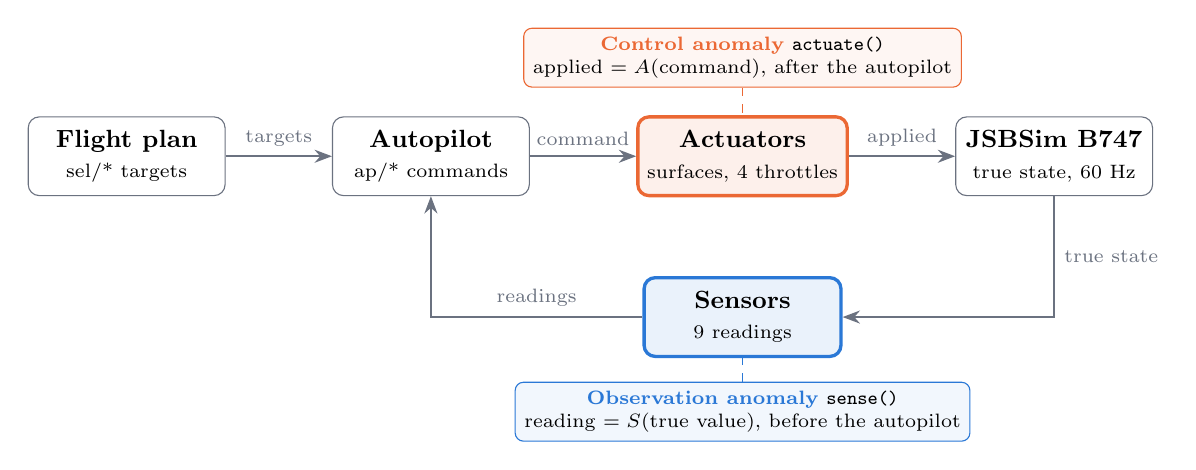
\begin{tikzpicture}[
      box/.style={draw=muted, rounded corners=4pt, minimum width=2.5cm, minimum height=1.0cm, align=center, font=\small},
      arr/.style={-{Stealth[length=2.2mm]}, draw=muted, thick},
      lab/.style={font=\scriptsize, text=muted}]
    \node[box] (plan) {\textbf{Flight plan}\\\scriptsize sel/* targets};
    \node[box, right=1.35cm of plan] (ap) {\textbf{Autopilot}\\\scriptsize ap/* commands};
    \node[box, right=1.35cm of ap, draw=twin, fill=twin!10, very thick] (act) {\textbf{Actuators}\\\scriptsize surfaces, 4 throttles};
    \node[box, right=1.35cm of act] (fdm) {\textbf{JSBSim B747}\\\scriptsize true state, 60 Hz};
    \node[box, below=1.0cm of act, draw=flight, fill=flight!10, very thick] (sen) {\textbf{Sensors}\\\scriptsize 9 readings};
    \draw[arr] (plan) -- node[lab, above] {targets} (ap);
    \draw[arr] (ap) -- node[lab, above] {command} (act);
    \draw[arr] (act) -- node[lab, above] {applied} (fdm);
    \draw[arr] (fdm.south) |- node[lab, pos=0.25, right] {true state} (sen.east);
    \draw[arr] (sen.west) -| node[lab, pos=0.25, above] {readings} (ap.south);
    \node[above=0.35cm of act, draw=twin, rounded corners=3pt, fill=twin!6, font=\scriptsize, align=center] (cn)
      {\ctl{Control anomaly} \texttt{actuate()}\\ applied $=A(\text{command})$, after the autopilot};
    \node[below=0.3cm of sen, draw=flight, rounded corners=3pt, fill=flight!6, font=\scriptsize, align=center] (on)
      {\obs{Observation anomaly} \texttt{sense()}\\ reading $=S(\text{true value})$, before the autopilot};
    \draw[twin, dashed] (cn) -- (act);
    \draw[flight, dashed] (on) -- (sen);
  \end{tikzpicture}
  \vspace{0.4em}

  \aside{The fault is injected \emph{inside} the loop: the autopilot reacts and the effect propagates through the physics.}
\end{frame}

% ================================================================ 6
\begin{frame}{One physics step (60 Hz) and what is logged (4 Hz)}
  \begin{columns}[T]
    \begin{column}{0.47\textwidth}
      \textbf{Every 1/60 s}
      \begin{enumerate}\small
        \item flight plan $\rightarrow$ selected ALT, CAS, HDG
        \item \obs{sensors} $\rightarrow$ 9 readings: ALT CAS VS PITCH ROLL HDG BETA Q P \hfill\texttt{sense()}
        \item autopilot $\rightarrow$ elevator, aileron, rudder, throttle
        \item \ctl{actuators} $\rightarrow$ applied commands \hfill\texttt{actuate()}
        \item JSBSim advances one step
      \end{enumerate}
    \end{column}
    \begin{column}{0.49\textwidth}
      \textbf{Every 15th step}
      \small
      \begin{tabularx}{\linewidth}{@{}l L@{}}
        \toprule
        \texttt{sensor/*} & what the autopilot \emph{read} (+ noise) \\
        \texttt{sensor/TLA1-4} & thrust-lever angles \\
        \texttt{ap/*} & commands \emph{before} control anomaly \\
        \texttt{sel/*} & flight plan \\
        \texttt{derived/egt} & EGT per engine \\
        JSBSim props & the \emph{true} state, $\sim$650 \\
        \texttt{label} & 1 while the fault acts \\
        \bottomrule
      \end{tabularx}
    \end{column}
  \end{columns}
  \vspace{0.8em}
  \aside{Logging reading, command, applied value and true state lets you see \emph{where} a fault entered.}
\end{frame}

% ================================================================ 7
\begin{frame}{Aircraft and why cruise only}
  \begin{columns}[T]
    \begin{column}{0.5\textwidth}
      \textbf{Aircraft}
      \begin{itemize}\small
        \item JSBSim's shipped \textbf{B747} model, copied as \texttt{B747P}
        \item + payload point mass (gross weight varies)
        \item + main tanks 10.9 $\rightarrow$ 25 klb (realistic cruise weight)
        \item trimmed at cruise, then a small random attitude/rate disturbance
        \item elevator sign \emph{measured}, not assumed
      \end{itemize}
    \end{column}
    \begin{column}{0.47\textwidth}
      \textbf{Why cruise}
      \begin{itemize}\small
        \item longest phase of flight
        \item near steady state $\rightarrow$ clean ground truth
        \item where industry trend monitoring is done
        \item no ground contact, gear, flaps or pilot inputs
        \item climb/descent: future work
      \end{itemize}
    \end{column}
  \end{columns}
  \vspace{0.8em}
  \begin{block}{}
    \small Why the B747: mature model, \textbf{four engines} (engine-vs-engine comparison is the key throttle-fault signature), continuity with earlier notebooks.
  \end{block}
\end{frame}

% ================================================================ 8
\begin{frame}{Normal variability: no two normal flights alike}
  \begin{columns}[T]
    \begin{column}{0.44\textwidth}
      \scriptsize
      \begin{tabularx}{\linewidth}{@{}l L@{}}
        \toprule
        length & 25--35 min \\
        altitude & 28--34 kft \\
        Mach & 0.705--0.735 \\
        turns & 0--3, $\pm$10--60$^\circ$ \\
        step climb & 30\,\%, +2000 ft \\
        Mach change & 30\,\%, $\pm$0.005--0.015 \\
        AP gains & each $\times$U(0.85, 1.15) \\
        ISA dev. & N(0, 5)\,$^\circ$C \\
        wind & 0--50 kt, veering \\
        turbulence & calm 25\,\% / light 75\,\% \\
        payload & 20--120 klb \\
        fuel & tanks 60--90\,\% \\
        \bottomrule
      \end{tabularx}\\[0.5em]
      \textbf{Hard normals} (labelled normal):\\ moderate turbulence, 70--100 kt wind, hot/cold day ($\pm$15--22\,$^\circ$C), heavy.
    \end{column}
    \begin{column}{0.54\textwidth}
      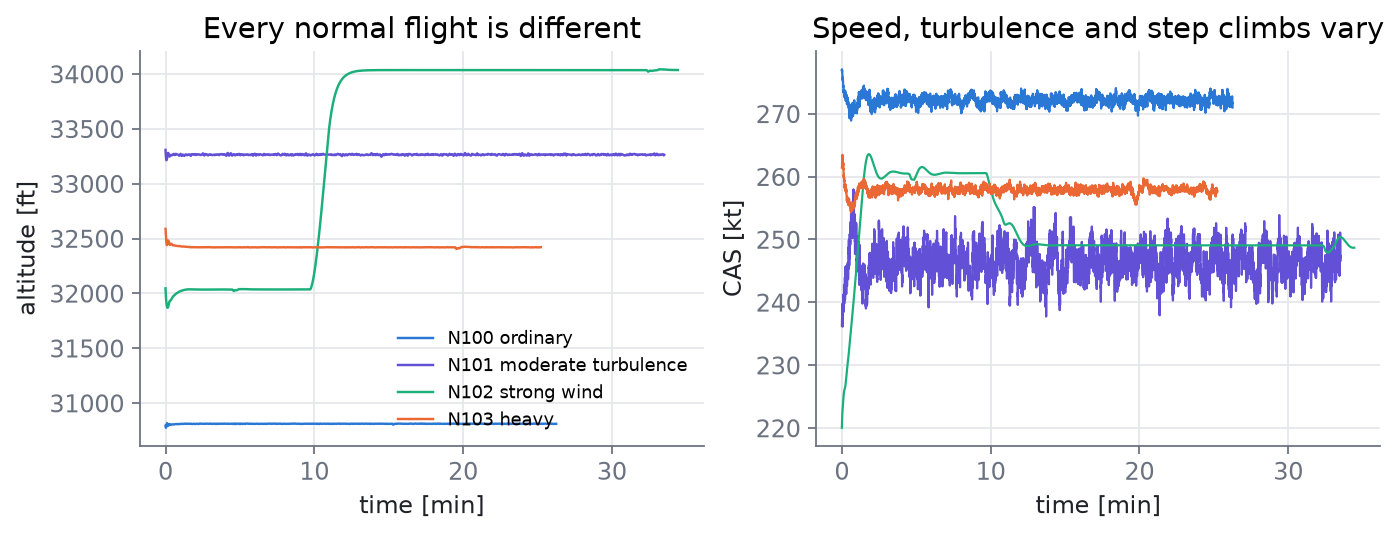
\includegraphics[width=\linewidth]{normals.png}\\
      \aside{Four demo normal flights: different levels, speeds, turbulence, a step climb.}
    \end{column}
  \end{columns}
\end{frame}

% ================================================================ 9
\begin{frame}{The autopilot: four classical loops}
  \small
  \textbf{Altitude $\rightarrow$ pitch $\rightarrow$ elevator}
  \[
    \dot h_{cmd} = \mathrm{clip}\big(2.0\,(h_{tgt} - \hat h)\big),\quad
    \theta_{cmd} = \theta_I + 0.0022(\dot h_{cmd} - \hat{\dot h}),\quad
    \delta_e = s_e\big(0.060(\theta_{cmd} - \hat\theta) - 1.5\,\hat q\big)
  \]
  \textbf{Speed $\rightarrow$ throttle} (PID, anti-windup, slew 0.055/s, same command to all 4 engines)
  \[
    e = \widehat{CAS} - CAS_{sel},\qquad u_{thr} = \mathrm{clip}\big(I - 0.020\,e - 0.020\,\dot{\widehat{CAS}},\ 0.18,\ 1\big)
  \]
  \textbf{Heading $\rightarrow$ bank $\rightarrow$ aileron} \qquad \textbf{Sideslip $\rightarrow$ rudder (PI)}
  \[
    \phi_{cmd} = \mathrm{clip}(1.2\,\Delta\hat\psi, \pm25^\circ),\ \ \delta_a = 0.020(\phi_{cmd} - \hat\phi) - 0.55\,\hat p
    \qquad
    \delta_r = -\big(0.03\,\hat\beta + 0.01\!\int\!\hat\beta\,dt\big)
  \]
  \vspace{0.2em}
  \aside{Hats = sensed values, each one can carry an observation anomaly. Custom autopilot because it must read through \texttt{sense()}; gains from the verified v2 notebooks.}
\end{frame}

% ================================================================ 10
\begin{frame}{Observation vs control anomalies}
  \small
  \begin{tabularx}{\textwidth}{@{}l L L@{}}
    \toprule
    & \obs{Observation} & \ctl{Control} \\
    \midrule
    What is wrong & what the autopilot \textbf{reads} & what the aircraft \textbf{receives} \\
    Autopilot decision & correct for the wrong reading & correct for the true state \\
    Aircraft & really moves off target & responds wrongly; autopilot compensates \\
    Faulty channel & often looks normal (held on target) & command $\neq$ applied / surface / engine \\
    Real examples & pitot blockage (Birgenair 301, Aeroperu 603) & jammed elevator, rudder runaway, fuel-control fault \\
    Classic name & sensor fault & actuator fault \\
    \bottomrule
  \end{tabularx}
  \vspace{1em}
  \begin{block}{}
    Key insight: for observation faults the \emph{faulty sensor is the least suspicious channel}. The evidence is in the true state and in other sensors.
  \end{block}
\end{frame}

% ================================================================ 11
\begin{frame}{Observation catalogue (6 types on 9 sensed variables)}
  \scriptsize
  \begin{tabularx}{\textwidth}{@{}l L l l@{}}
    \toprule
    Type & Injection & Profiles & Max dur. \\
    \midrule
    \texttt{sensor\_bias} & reading $=$ true $+ s\,m\,g(t)$ & step, intermittent & 900 s \\
    \texttt{sensor\_drift} & reading $=$ true $+ s\,2m\,(t-t_0)/(t_{end}-t_0)$ & ramp & 900 s \\
    \texttt{sensor\_stuck} & reading $=$ true$(t_0)$, frozen & step & 180 s \\
    \texttt{sensor\_noise} & reading $=$ true $+\,\mathcal N(0,(m/2)^2)$ every 1/60 s & step, intermittent & 600 s \\
    \texttt{sensor\_spikes} & reading $=$ true $\pm 3m$, spikes 0.25--1 s, $\sim$4/min & step & 600 s \\
    \texttt{pitot\_blockage} & $p_t$ frozen; $\widehat{CAS}=\mathrm{CAS}\big(p_t^* - p_s(h)\big)$ & step & 300 s \\
    \bottomrule
  \end{tabularx}
  \vspace{0.6em}

  \begin{tabularx}{\textwidth}{@{}l *{7}{>{\centering\arraybackslash}X}@{}}
    \toprule
    Limits & ALT ft & CAS kt & VS fpm & PITCH/ROLL$^\circ$ & HDG$^\circ$ & BETA$^\circ$ & Q, P $^\circ$/s \\
    \midrule
    bias, drift & 50--400 & 3--15 & 150--600 & 0.5--3 & 2--15 & 0.3--2 & 0.11--0.57 \\
    noise, spikes & 20--150 & 1--6 & 100--400 & 0.2--1.5 & 0.5--4 & 0.1--0.8 & 0.06--0.34 \\
    \bottomrule
  \end{tabularx}
  \vspace{0.4em}
  \aside{Lower limit $\approx$ normal noise/turbulence level (hard); upper limit clearly abnormal but flyable.}
\end{frame}

% ================================================================ 12
\begin{frame}{Control catalogue (5 surface + 3 throttle types)}
  \scriptsize
  \begin{tabularx}{\textwidth}{@{}l L l l@{}}
    \toprule
    Type & Injection (on command $u$) & Profiles & Max dur. \\
    \midrule
    \texttt{surface\_bias} & $u + s\,m\,g(t)$ & step, ramp, interm. & 900 s \\
    \texttt{surface\_stuck} & $u(t_0)$, frozen & step & 120 s elev., 600 s \\
    \texttt{surface\_loss\_of\_eff.} & $u\,(1 - m\,g(t))$ & step, ramp & 900 s \\
    \texttt{surface\_oscillation} & $u + m\,g(t)\sin 2\pi f (t-t_0)$, $f\sim U(0.3,1.5)$ Hz & step, interm. & 600 s \\
    \texttt{surface\_runaway} & $u + s\,m\,\min(1, (t-t_0)/30\,\mathrm{s})$ & step & 300 s \\
    \texttt{throttle\_thrust\_loss} & $u_e(1 - m\,g(t))$, one engine & step, ramp, interm. & 900 s \\
    \texttt{throttle\_lever\_stuck} & $u_e(t_0)$, frozen, lever shows it & step & 900 s \\
    \texttt{throttle\_lever\_bias} & $u_e + s\,m\,g(t)$ & step, ramp & 900 s \\
    \bottomrule
  \end{tabularx}
  \vspace{0.6em}

  \begin{tabularx}{\textwidth}{@{}l *{4}{>{\centering\arraybackslash}X}@{}}
    \toprule
    Limits & elevator & aileron & rudder & engine \\
    \midrule
    bias & 0.02--0.10 & 0.02--0.15 & 0.02--0.15 & 0.03--0.15 \\
    loss (fraction) & 0.15--0.5 & 0.2--0.7 & 0.2--0.7 & 0.05--0.40 \\
    oscillation & 0.01--0.04 & 0.01--0.06 & 0.01--0.06 & --- \\
    runaway & 0.03--0.12 & 0.05--0.25 & 0.05--0.25 & --- \\
    \bottomrule
  \end{tabularx}
  \vspace{0.3em}
  \aside{Surface units $-1\dots1$ ($\approx20^\circ$ per unit); throttle $0\dots1$. Elevator jam capped at 120 s: longer leaves a realistic envelope.}
\end{frame}

% ================================================================ 13
\begin{frame}{Sampling one anomaly: how strong, when, how long}
  \footnotesize
  \begin{columns}[T]
    \begin{column}{0.5\textwidth}
      \[ m = m_{lo}\Big(\tfrac{m_{hi}}{m_{lo}}\Big)^{s},\quad s\sim U(0,1) \]
      \[ t_0 \sim U(300\,\mathrm{s},\ T - 420\,\mathrm{s}) \]
      \[ d = \mathrm{clip}\big(e^{\mathcal N(\ln 300,\,0.6^2)},\ 60,\ \min(d_{max}, T-120-t_0)\big) \]
    \end{column}
    \begin{column}{0.47\textwidth}
      \begin{itemize}\footnotesize
        \item \textbf{log-uniform}: each factor 2 equally likely, small faults as common as large
        \item \textbf{onset} after the 5-min start transient, 2-min recovery tail, no fixed position to learn
        \item \textbf{log-normal}: positive, skewed; middle 68\,\% $\approx$ 2.7--9 min
        \item \textbf{profiles}: step 0.5, ramp 0.3, intermittent 0.2 (bursts 20--60 s on, 30--120 s off)
      \end{itemize}
    \end{column}
  \end{columns}
  \vspace{0.3em}
  \centering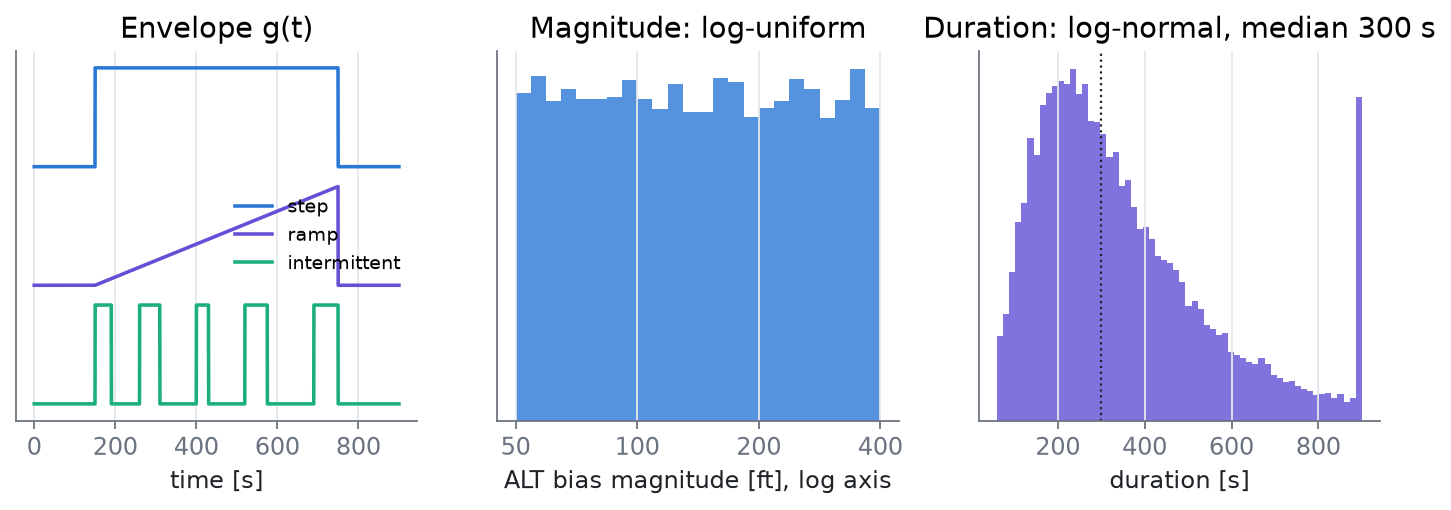
\includegraphics[width=0.66\textwidth]{sampling.png}
\end{frame}

% ================================================================ 14
\begin{frame}{Example 1 --- observation: altitude sensor bias (O100)}
  \begin{columns}[c]
    \begin{column}{0.58\textwidth}
      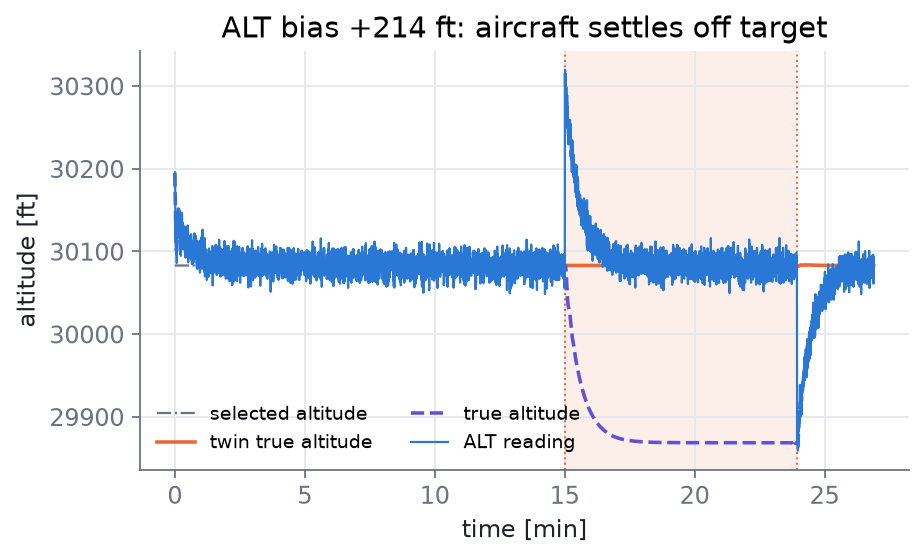
\includegraphics[width=\linewidth]{altbias_O100.png}
    \end{column}
    \begin{column}{0.40\textwidth}
      \small
      \begin{itemize}\setlength\itemsep{0.5em}
        \item Bias $+214$ ft, step, 900--1436 s.
        \item The autopilot drives the \textcolor{flight}{\textbf{reading}} back to the target.
        \item So the \textcolor{truth}{\textbf{true altitude}} settles 214 ft \emph{low}.
        \item The reading looks normal --- only the jump at onset and end gives it away.
        \item \textcolor{twin}{\textbf{Twin}} shows where the aircraft should be.
      \end{itemize}
    \end{column}
  \end{columns}
\end{frame}

% ================================================================ 15
\begin{frame}{Example 2 --- observation: pitot blockage (O105)}
  \centering
  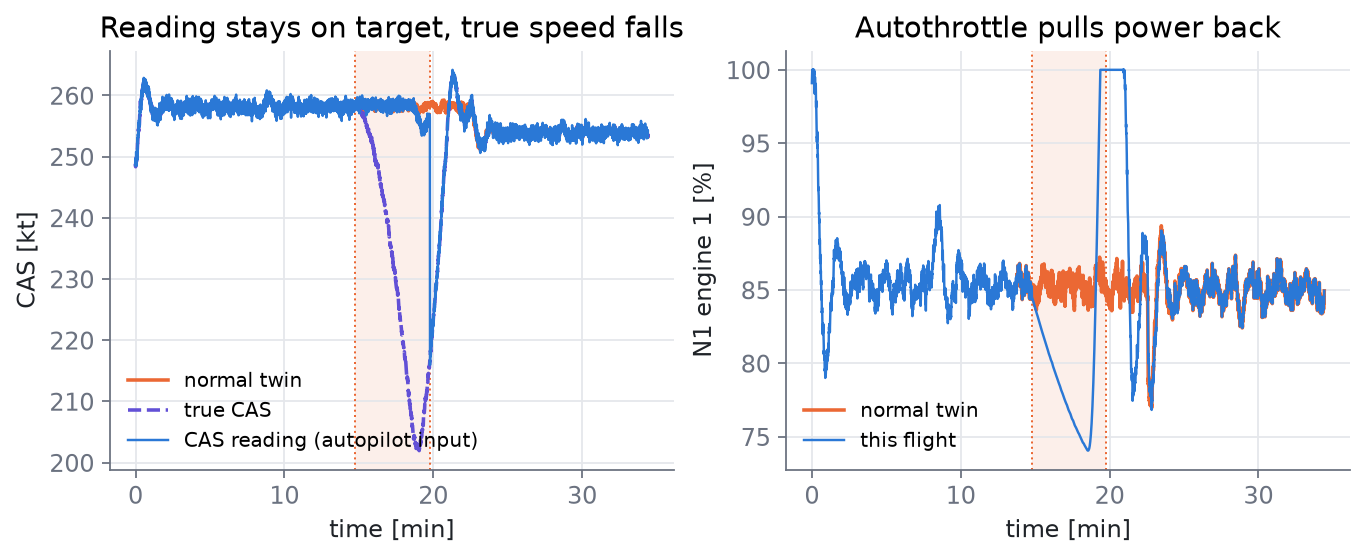
\includegraphics[width=0.92\textwidth]{pitot_O105.png}
  \vspace{0.3em}

  \small
  Total pressure frozen at onset $\Rightarrow$ indicated CAS depends only on altitude. The autothrottle holds the frozen reading,
  pulls power back, and the \textcolor{truth}{\textbf{true speed}} falls $\sim$55 kt in 5 min. Mechanism of Birgenair 301 / Aeroperu 603.
\end{frame}

% ================================================================ 16
\begin{frame}{Example 3 --- control: elevator stuck (C101)}
  \centering
  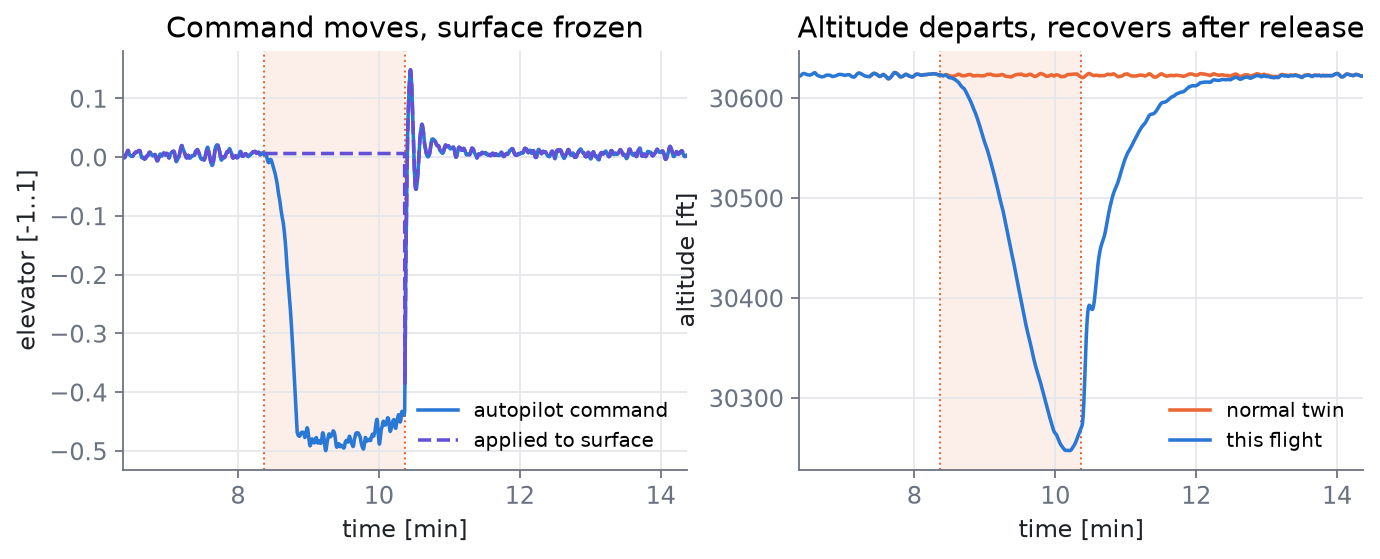
\includegraphics[width=0.92\textwidth]{elevstuck_C101.png}
  \vspace{0.3em}

  \small
  The surface freezes at its onset position. The autopilot keeps commanding (down to $-0.47$) but nothing moves; altitude drops
  $\sim$380 ft. On release the loop recovers. The signature: \textbf{command $\neq$ applied}.
\end{frame}

% ================================================================ 17
\begin{frame}{Example 4 --- control: thrust loss on engine 2 (C105)}
  \centering
  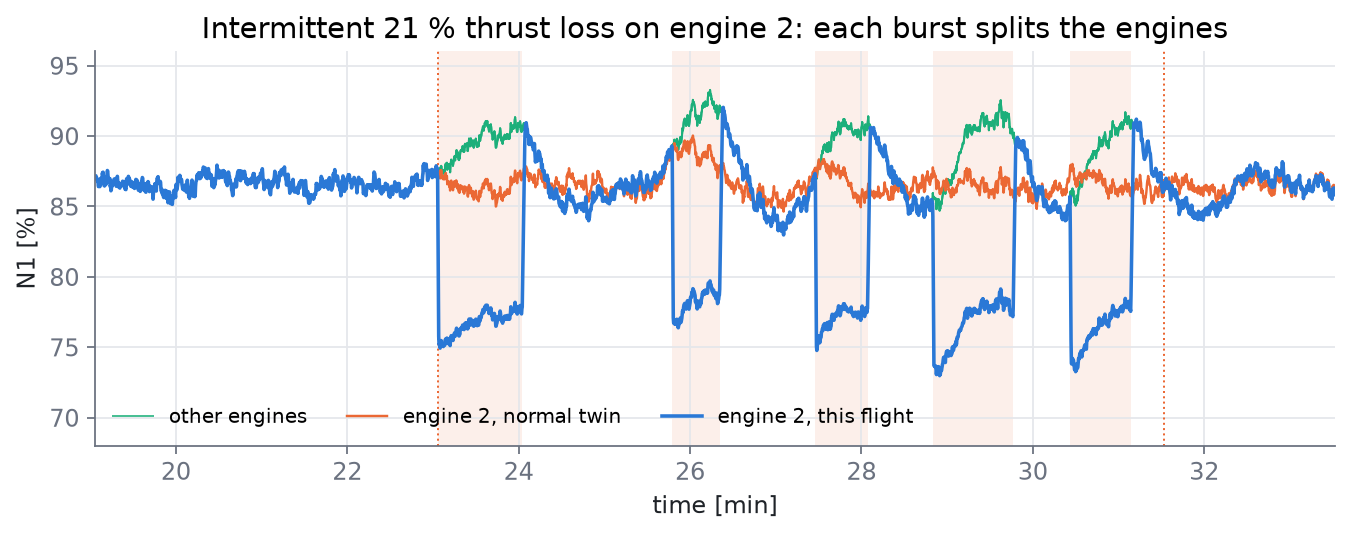
\includegraphics[width=0.9\textwidth]{thrustloss_C105.png}
  \vspace{0.3em}

  \small
  21\,\% thrust loss in five bursts. Engine 2's N1 drops; the autothrottle pushes the \textcolor{other}{\textbf{other three engines}} up to hold speed.
  The lever (TLA) looks normal. The signature: \textbf{engine-to-engine split}.
\end{frame}

% ================================================================ 18
\begin{frame}{What is logged: 680 channels, 329 change in flight}
  \begin{columns}[T]
    \begin{column}{0.5\textwidth}
      \small
      \textbf{Why log everything}
      \begin{itemize}\footnotesize
        \item effects spread into channels nobody would pre-select (rudder runaway $\rightarrow$ yawing moment, lateral acceleration)
        \item a realistic recorder subset can be chosen later without regenerating
      \end{itemize}
      \textbf{Why 4 Hz}
      \begin{itemize}\footnotesize
        \item typical recorder rate for these parameters (DASHlink 0.25--16 Hz)
        \item 60 Hz = 15$\times$ size, no extra information in cruise
      \end{itemize}
      \textbf{Excluded}
      \begin{itemize}\footnotesize
        \item \texttt{gear/*}, \texttt{ground/*}: meaningless in cruise, some hold uninitialised memory (1e180)
      \end{itemize}
    \end{column}
    \begin{column}{0.47\textwidth}
      \footnotesize
      \begin{tabularx}{\linewidth}{@{}L r@{}}
        \toprule
        Subsystem & changing / logged \\
        \midrule
        Engines 1--4 & 52 / 160 \\
        Aerodynamics & 42 / 50 \\
        Velocities \& rates & 40 / 40 \\
        Position & 30 / 30 \\
        Flight controls & 26 / 58 \\
        Atmosphere \& wind & 24 / 55 \\
        Accelerations, forces, moments & 54 / 64 \\
        Sensors, AP, plan & 18 / 18 \\
        Other (fuel, mass, earth, ...) & 43 / 205 \\
        \midrule
        \textbf{Total} & \textbf{329 / 680} \\
        \bottomrule
      \end{tabularx}\\[0.4em]
      \aside{Measurement noise on \texttt{sensor/*}: ALT 10 ft, CAS 0.5 kt, VS 30 fpm, attitude 0.05$^\circ$.}
    \end{column}
  \end{columns}
\end{frame}

% ================================================================ 19
\begin{frame}{The normal twin and the labels}
  \begin{columns}[T]
    \begin{column}{0.52\textwidth}
      \small
      \textbf{Normal twin} = same seed, same weather, same turbulence, same sensor noise, \emph{no anomaly}.
      \begin{itemize}\footnotesize
        \item separate seeded random streams: scenario (seed), anomaly (+7), noise (+11), anomaly noise (+99), turbulence
        \item removing the anomaly changes nothing else
        \item \textbf{identical before onset}: max difference = 0 over all channels, all 16 demo twins
        \item stored from onset $-$ 60 s to the end
      \end{itemize}
    \end{column}
    \begin{column}{0.45\textwidth}
      \small
      \textbf{Labels} (per 4 Hz row)
      \[ \mathrm{label}(t) = \mathbf 1\big[t_0 \le t < t_{end}\big]\ (\wedge\ \text{in a burst}) \]
      \begin{itemize}\footnotesize
        \item 1 while the fault \emph{acts}
        \item recovery after the end is labelled 0
        \item intermittent: 1 only during bursts
      \end{itemize}
    \end{column}
  \end{columns}
  \vspace{0.8em}
  \begin{block}{}
    \small Without the twin, a difference between a faulty and a normal flight mixes the fault with weather, weight and route. With it, every difference \emph{is} the fault.
  \end{block}
\end{frame}

% ================================================================ 20
\begin{frame}{Effect score: where does each anomaly show?}
  \small
  \[
    \sigma_c = \max\big(\mathrm{std}(y_c),\ 10^{-3}|\bar y_c|,\ 0.05\,\mathrm{std}(x_c)\big),\qquad
    \mathrm{score}_c = \max_{t\ge t_0}\frac{|x_c(t)-y_c(t)|}{\sigma_c}
  \]
  \aside{$x$ = flight, $y$ = twin. Floors stop near-constant channels from scoring $10^{14}$. Capped at 999.}
  \vspace{0.6em}

  \begin{tabularx}{\textwidth}{@{}l l L@{}}
    \toprule
    Role & Rule & Meaning \\
    \midrule
    injection point & where the hook acts & \texttt{sensor/X}, \texttt{fcs/<surface>-cmd-norm}, engine throttle + TLA \\
    strong & score $\ge 3$ & departs by $>$3 normal spreads \\
    moderate & $1 \le$ score $< 3$ & clearly visible against the twin \\
    weak & $0.25 \le$ score $< 1$ & visible only overlaid on the twin \\
    \bottomrule
  \end{tabularx}
  \vspace{0.8em}
  \begin{block}{}
    \small This is a \textbf{verification tool, not a detector}: it uses the twin, which reality never has.
  \end{block}
\end{frame}

% ================================================================ 21
\begin{frame}{Verification}
  \begin{columns}[c]
    \begin{column}{0.36\textwidth}
      \scriptsize
      \begin{itemize}\setlength\itemsep{0.35em}
        \item twin identical before onset: \textbf{0 difference}, 16/16
        \item same seed $\Rightarrow$ same flight
        \item each injection matches its formula (plotted)
        \item 20/20 demo flights complete, autopilot stable
        \item effects physically sensible chains
        \item $\sim$7 s per 30-min flight; demo set $\approx$ 1 min on 6 cores
      \end{itemize}
      \vspace{0.4em}
      \aside{Weak cases are physics, not bugs: elevator loss of effectiveness matters only for large commands; a stuck lever only if the autothrottle moves.}
    \end{column}
    \begin{column}{0.62\textwidth}
      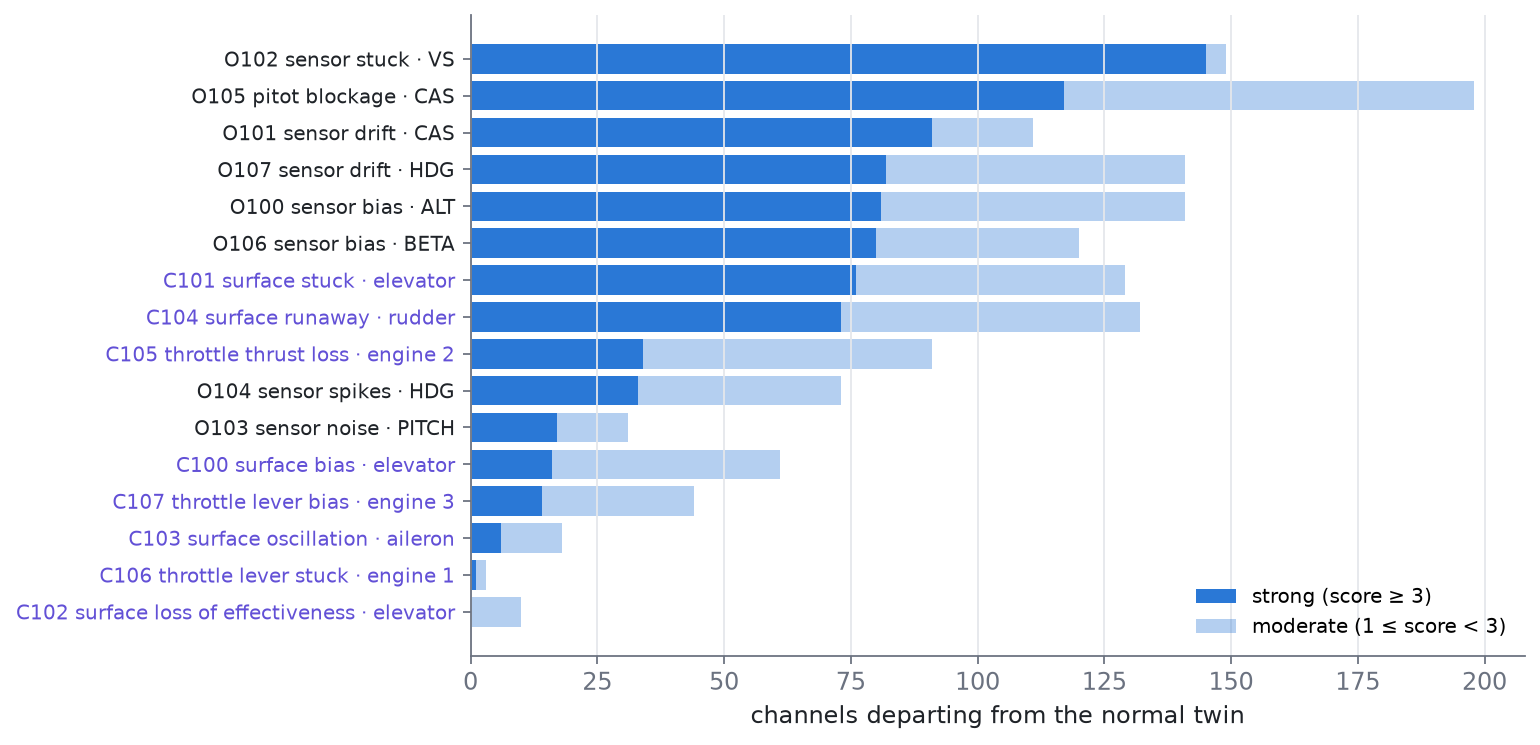
\includegraphics[width=\linewidth]{effects.png}\\
      \aside{Channels departing from the twin per demo flight (severity 0.7). Control flights in violet.}
    \end{column}
  \end{columns}
\end{frame}

% ================================================================ 22
\begin{frame}{The viewer}
  \begin{columns}[c]
    \begin{column}{0.58\textwidth}
      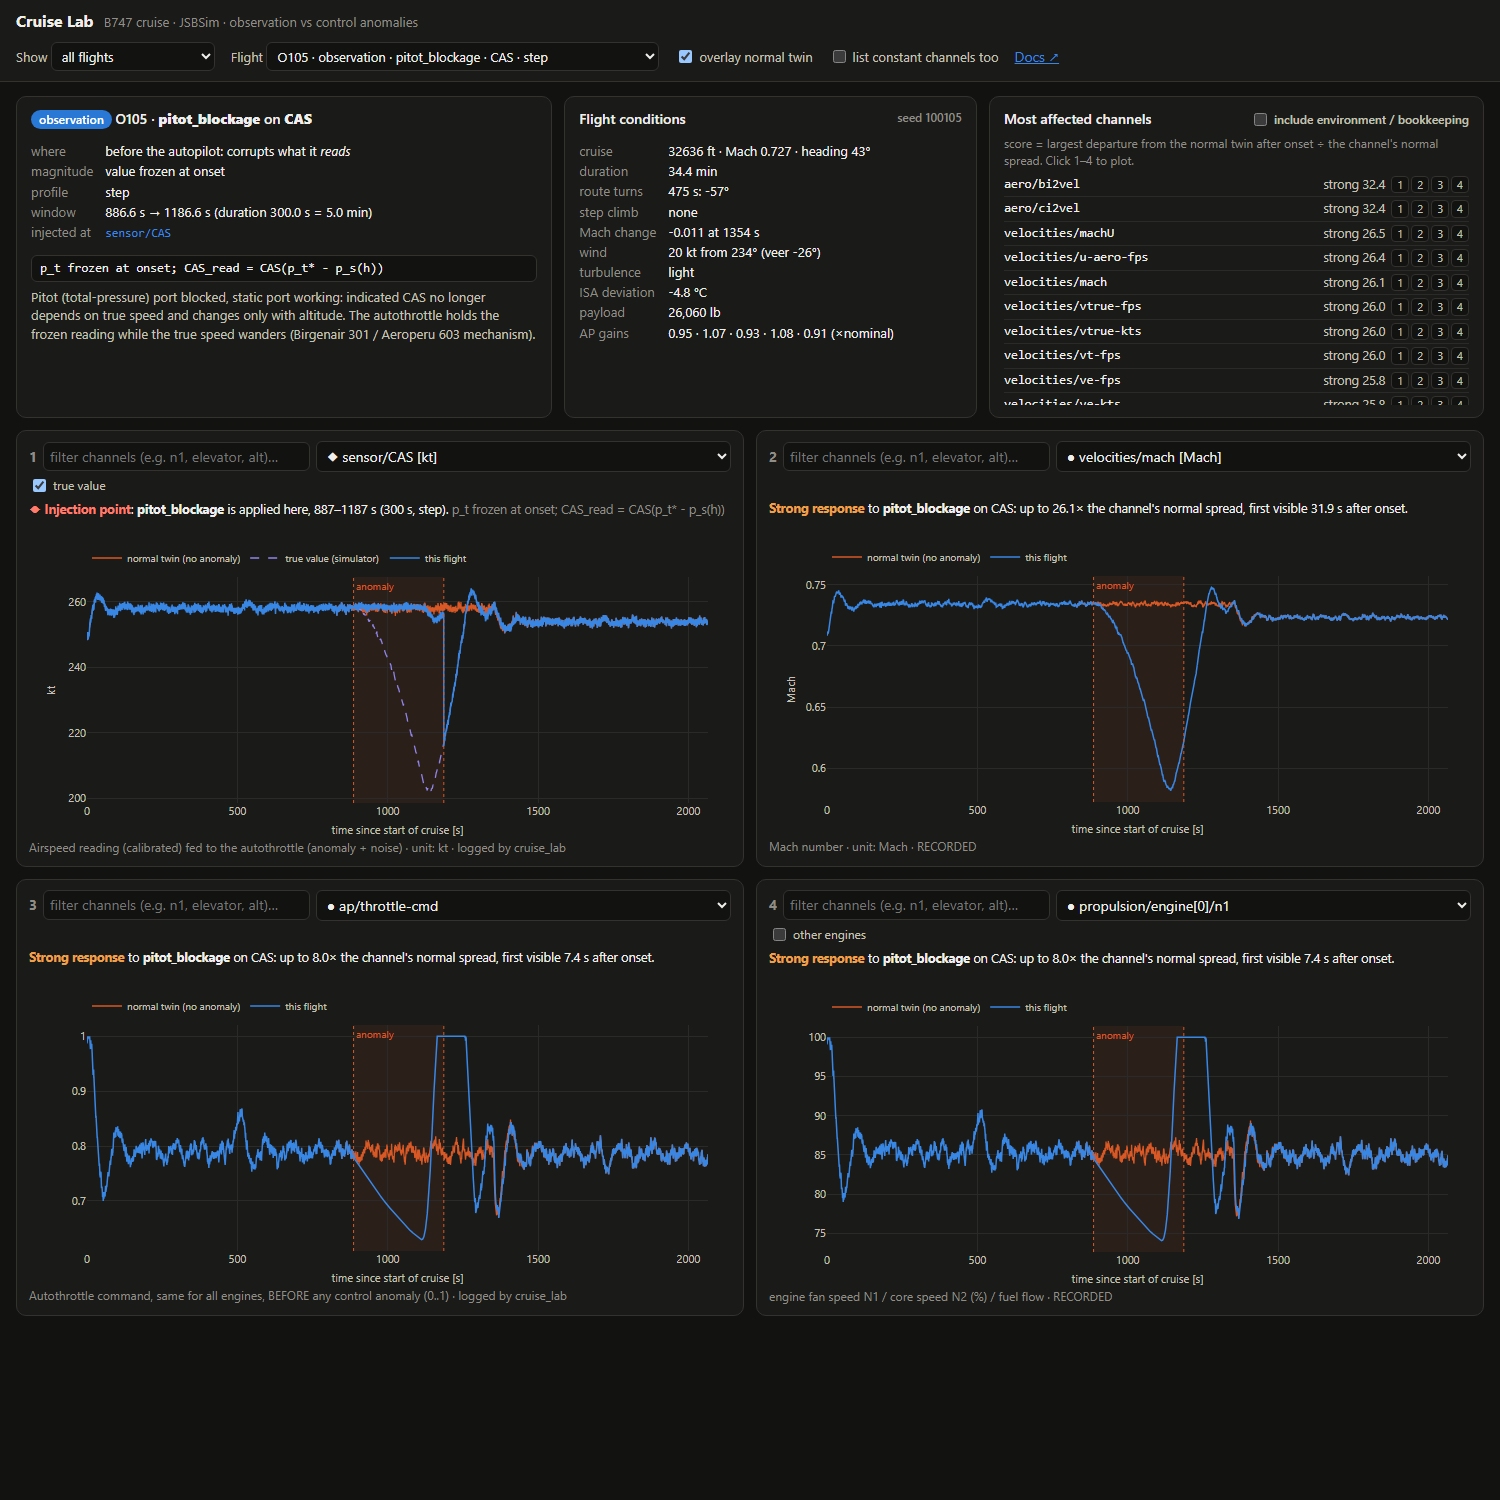
\includegraphics[width=\linewidth]{viewer_O105.png}
    \end{column}
    \begin{column}{0.40\textwidth}
      \footnotesize
      \begin{itemize}\setlength\itemsep{0.35em}
        \item flight drop-down, filter by kind
        \item anomaly card: type, target, magnitude, window, formula
        \item flight conditions + most-affected channels
        \item \textbf{four panels}, any of 329 channels, grouped by subsystem
        \item overlays: \textcolor{twin}{twin}, \textcolor{truth}{true value}, \textcolor{other}{other engines}
        \item role line per channel; linked zoom
      \end{itemize}
      \vspace{0.4em}
      \texttt{python viewer\textbackslash server.py}\\ $\rightarrow$ \texttt{localhost:8050}
    \end{column}
  \end{columns}
\end{frame}

% ================================================================ 23
\begin{frame}{Design decisions --- and why not the alternative}
  \scriptsize
  \begin{tabularx}{\textwidth}{@{}l l L@{}}
    \toprule
    Decision & Chosen & Rejected alternative --- why \\
    \midrule
    Where to inject & inside the loop & post-hoc edit of logs: nothing reacts, artefact is learnable \\
    Faults per flight & one & several: confounded labels (later extension) \\
    Magnitude & log-uniform & uniform: biased to large, easy faults \\
    Onset & U(300 s, T$-$420 s) & fixed: leaks the answer; at $t=0$: mixed with start transient \\
    Duration & log-normal, capped & fixed: unrealistic, learnable \\
    Profiles & step, ramp, intermittent & step only: overstates detectability \\
    Counterfactual & twin, same seed & another normal flight: weather/weight swamp the fault \\
    Randomness & separate seeded streams & one RNG: twin diverges from $t=0$ \\
    Logging & all props, 4 Hz & 20 picked channels: misses effects \\
    Format & Parquet float32 zstd & CSV: 5--10$\times$ larger, slow \\
    Hard normals & 5 conditions & none: ``unusual = faulty'' would look perfect \\
    Viewer & local web, linked panels & static PNGs: cannot cover 329 channels \\
    \bottomrule
  \end{tabularx}
\end{frame}

% ================================================================ 24
\begin{frame}{Limitations (stated openly)}
  \small
  \begin{itemize}\setlength\itemsep{0.45em}
    \item \textbf{Model fidelity}: table-based aero, simplified turbine (no component efficiencies). Plausible, not certified.
    \item \textbf{Autopilot simpler than real}: no FMS modes, no envelope protection, no pilot, no disconnect logic.
    \item \textbf{Noise outside the loop}: the autopilot reads true + anomaly; measurement noise is added to logs only.
    \item \textbf{No sensor redundancy}: real aircraft vote between 2--3 sensors.
    \item \textbf{Minimal recorder model}: no quantization, mixed rates or dropouts yet.
    \item \textbf{Scope}: cruise only, one fault per flight, 25--35 min.
    \item \textbf{Limits and noise levels are engineering judgement}, not failure statistics.
  \end{itemize}
\end{frame}

% ================================================================ 25
\begin{frame}{Next steps}
  \begin{enumerate}\setlength\itemsep{0.5em}
    \item Generate the \texttt{catalog} (every type $\times$ variable) and a large \texttt{random} set with train / validation / test splits.
    \item Recorder realism: 12-bit quantization, mixed sample rates, natural dropouts in every flight.
    \item Measurement noise inside the loop.
    \item Leakage checks: simple thresholds must \emph{not} find everything (Wu \& Keogh).
    \item Climb and descent; engine-performance faults (N-CMAPSS style).
    \item FlightGear replay of selected flights.
    \item \emph{Then} detectors (autoencoder, Isolation Forest, MKAD-style), evaluated with PR-AUC, false alarms per flight, detection delay.
  \end{enumerate}
\end{frame}

% ================================================================ 26
\begin{frame}{Summary}
  \begin{columns}[T]
    \begin{column}{0.48\textwidth}
      \begin{itemize}\setlength\itemsep{0.6em}
        \item Closed-loop JSBSim B747 cruise, 60 Hz physics, 4 Hz logs
        \item \obs{6 observation} + \ctl{8 control} anomaly types, injected inside the loop
        \item Magnitude, onset, duration and profile randomised with stated distributions
      \end{itemize}
    \end{column}
    \begin{column}{0.48\textwidth}
      \begin{itemize}\setlength\itemsep{0.6em}
        \item Normal twin per anomaly: exact counterfactual, verified identical before onset
        \item 680 channels (329 changing), labels, metadata
        \item Viewer + docs to inspect any flight and any channel
      \end{itemize}
    \end{column}
  \end{columns}
  \vspace{2em}
  \centering{\Large Questions?}\\[0.6em]
  \aside{Live demo: \texttt{localhost:8050} \textbullet{} docs: \texttt{cruise\_lab/docs} \textbullet{} maths: \texttt{anomaly\_injection.pdf}}
\end{frame}

% ================================================================ backup
\appendix
\begin{frame}{Backup: pitot blockage, the formula}
  \small
  At onset $t_0$, with static pressure $p_s(h)$ from the ISA model and impact pressure $q_c$:
  \[ p_t^* = p_s(h_0) + p_0\Big[\big(1 + 0.2\,(CAS_0/a_0)^2\big)^{3.5} - 1\Big] \]
  After onset:
  \[ q_c(t) = \max\big(p_t^* - p_s(h(t)),\,0\big),\qquad \widehat{CAS}(t) = a_0\sqrt{5\Big[\big(q_c/p_0+1\big)^{2/7}-1\Big]} \]
  \aside{$p_0 = 2116.2$ lbf/ft$^2$, $a_0 = 661.5$ kt. Climb $\Rightarrow p_s$ falls $\Rightarrow$ reading rises (and vice versa), regardless of true speed.}
\end{frame}

\begin{frame}{Backup: files and how to run}
  \small
  \begin{tabularx}{\textwidth}{@{}l L@{}}
    \toprule
    \texttt{python -m lab.generate} & demo set: 4 normal + 8 observation + 8 control, $\sim$1 min, 333 MB \\
    \texttt{-{}-preset catalog} & every type $\times$ variable + 10 normal, $\sim$4 min, $\sim$1.3 GB \\
    \texttt{-{}-preset random -{}-n N} & random draws, 1/3 each kind \\
    \texttt{python viewer\textbackslash server.py} & viewer at \texttt{localhost:8050} \\
    \midrule
    \texttt{flights/<id>.parquet} & one flight, 4 Hz, float32, zstd, $\sim$12 MB \\
    \texttt{flights/<id>\_twin.parquet} & normal twin from onset $-$ 60 s \\
    \texttt{meta/<id>.json} & scenario, anomaly, effects, twin check \\
    \texttt{manifest.json}, \texttt{channels.json} & index of flights and channels \\
    \bottomrule
  \end{tabularx}
\end{frame}

\begin{frame}{Backup: the 16 demo anomalies}
  \scriptsize
  \begin{tabularx}{\textwidth}{@{}l l l L l@{}}
    \toprule
    Flight & Type & Target & Magnitude & Window [s] \\
    \midrule
    O100 & sensor bias & ALT & +214 ft, step & 900--1436 \\
    O101 & sensor drift & CAS & $-$9.3 kt (to $-$18.5), ramp & 717--1065 \\
    O102 & sensor stuck & VS & frozen & 683--863 \\
    O103 & sensor noise & PITCH & sd 0.41$^\circ$ & 636--790 \\
    O104 & sensor spikes & HDG & $\pm$6.4$^\circ$ spikes & 678--856 \\
    O105 & pitot blockage & CAS & frozen $p_t$ & 887--1187 \\
    O106 & sensor bias & BETA & $-$1.13$^\circ$, intermittent & 965--1265 \\
    O107 & sensor drift & HDG & $-$8.2$^\circ$ (to $-$16.4), ramp & 576--1094 \\
    C100 & surface bias & elevator & $-$0.062 & 501--612 \\
    C101 & surface stuck & elevator & frozen & 502--622 \\
    C102 & loss of effectiveness & elevator & 35\,\% lost & 1495--1805 \\
    C103 & surface oscillation & aileron & 0.035 amplitude & 432--846 \\
    C104 & surface runaway & rudder & +0.154 & 405--705 \\
    C105 & thrust loss & engine 2 & 21\,\%, intermittent & 1383--1892 \\
    C106 & lever stuck & engine 1 & frozen & 342--504 \\
    C107 & lever bias & engine 3 & +0.093 & 565--712 \\
    \bottomrule
  \end{tabularx}
\end{frame}

\end{document}
